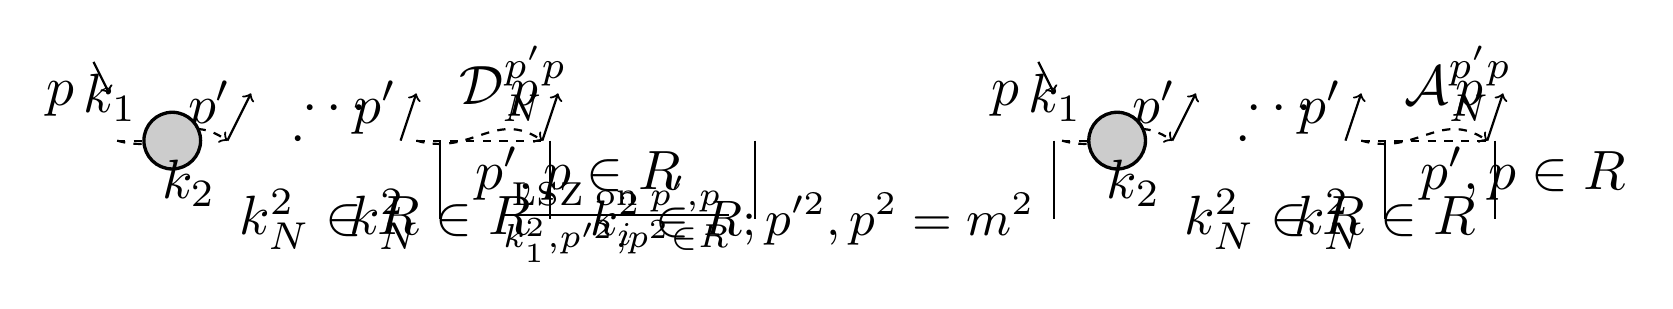
\begin{tikzpicture}[scale=2, every node/.style={transform shape}]
	\begin{scope}[xshift=-3cm]
	\draw[->, thick] (-1.5,0) -- (-1.4,-0.2);
	\node[anchor=north east, black] at (-1.5,0) {$p$};
	\draw[dashed,thick] (-1.35,-0.5)--(-1.05,-0.5);
	\draw[->,dashed,thick] (-1.35,-0.5) .. controls (-1,-0.6) and (-0.95,-0.3) .. (-0.65,-0.5);
	\draw[->,thick] (-0.65,-0.5) -- (-0.5,-0.2);
	\node[anchor=north east, black] at (-0.5,0) {$p'$};
	\filldraw[draw=black, fill=gray!40!white, very thick] (-1,-0.5) circle (0.18);
	\node[anchor=south east, black] at (-1.1,-0.5) {$k_1$};
	\node[anchor=north east, black] at (-0.6,-0.5) {$k_2$};
	\foreach \x in {-0.2,...,0.7}
	{
		\node[anchor=center, black] at (\x,-0.5) {$\cdot$};
	}
	\node[anchor=south west, black] at (-0.3,-0.5) {$\cdots$};
	\draw[->,thick] (0.45,-0.5) -- (0.55,-0.2);
	\node[anchor=north east, black] at (0.55,0) {$p'$};
	\draw[dashed,thick] (0.55,-0.5)--(1.35,-0.5);
	\draw[->,dashed,thick] (0.55,-0.5) .. controls (0.9,-0.6) and (1.05,-0.3) .. (1.35,-0.5);
	\draw[->,thick] (1.35,-0.5) -- (1.45,-0.2);
	\node[anchor=north east, black] at (1.45,0) {$p$};
	\draw[thick] (0.7,-0.5) -- (0.7,-1);
	\node[anchor=east, black] at (0.7,-1) {$k_N^2\in\mathbb{R}$};
	\draw[thick] (1.4,-0.5) -- (1.4,-1);
	\node[anchor=east, black] at (1.4,-1) {$k_N^2\in\mathbb{R}$};
	\node[anchor=south west, black] at (0.7,-0.5) {$\mathcal{D}^{p'p}_{N}$};
	\node[anchor=south west, black] at (0.8,-1) {$p',p\in\mathbb{R}$};
	\end{scope}
	\draw[thick] (-0.3,-0.5) -- (-0.3,-1);
	\node[anchor=east, black] at (-0.3,-1) {\small$\frac{\mathrm{LSZ\;on\;}p',p}{k_1^2,p'^2,p^2\in\mathbb{R}}$};
	\draw[thick] (1.6,-0.5) -- (1.6,-1);
	\node[anchor=east, black] at (1.6,-1) {\small$k_i^2\in\mathbb{R};p'^2,p^2=m^2$};
	\begin{scope}[xshift=3cm]
	\draw[->, thick] (-1.5,0) -- (-1.4,-0.2);
	\node[anchor=north east, black] at (-1.5,0) {$p$};
	\draw[dashed,thick] (-1.35,-0.5)--(-1.05,-0.5);
	\draw[->,dashed,thick] (-1.35,-0.5) .. controls (-1,-0.6) and (-0.95,-0.3) .. (-0.65,-0.5);
	\draw[->,thick] (-0.65,-0.5) -- (-0.5,-0.2);
	\node[anchor=north east, black] at (-0.5,0) {$p'$};
	\filldraw[draw=black, fill=gray!40!white, very thick] (-1,-0.5) circle (0.18);
	\node[anchor=south east, black] at (-1.1,-0.5) {$k_1$};
	\node[anchor=north east, black] at (-0.6,-0.5) {$k_2$};
	\foreach \x in {-0.2,...,0.7}
	{
		\node[anchor=center, black] at (\x,-0.5) {$\cdot$};
	}
	\node[anchor=south west, black] at (-0.3,-0.5) {$\cdots$};
	\draw[->,thick] (0.45,-0.5) -- (0.55,-0.2);
	\node[anchor=north east, black] at (0.55,0) {$p'$};
	\draw[dashed,thick] (0.55,-0.5)--(1.35,-0.5);
	\draw[->,dashed,thick] (0.55,-0.5) .. controls (0.9,-0.6) and (1.05,-0.3) .. (1.35,-0.5);
	\draw[->,thick] (1.35,-0.5) -- (1.45,-0.2);
	\node[anchor=north east, black] at (1.45,0) {$p$};
	\draw[thick] (0.7,-0.5) -- (0.7,-1);
	\node[anchor=east, black] at (0.7,-1) {$k_N^2\in\mathbb{R}$};
	\draw[thick] (1.4,-0.5) -- (1.4,-1);
	\node[anchor=east, black] at (1.4,-1) {$k_N^2\in\mathbb{R}$};
	\node[anchor=south west, black] at (0.7,-0.5) {$\mathcal{A}^{p'p}_{N}$};
	\node[anchor=south west, black] at (0.8,-1) {$p',p\in\mathbb{R}$};
	\end{scope}
	\end{tikzpicture}